\documentclass[11pt]{article}
\usepackage[a4paper,margin=1in]{geometry}
\usepackage{kotex}
\usepackage{amsmath}
\usepackage{booktabs}
\usepackage{array}
\usepackage{graphicx}
\usepackage{siunitx}
\usepackage{caption}
\usepackage{pdfpages}

\sisetup{
  group-separator={,},
  group-minimum-digits=4,
  round-mode=places,
  round-precision=1
}

\begin{document}

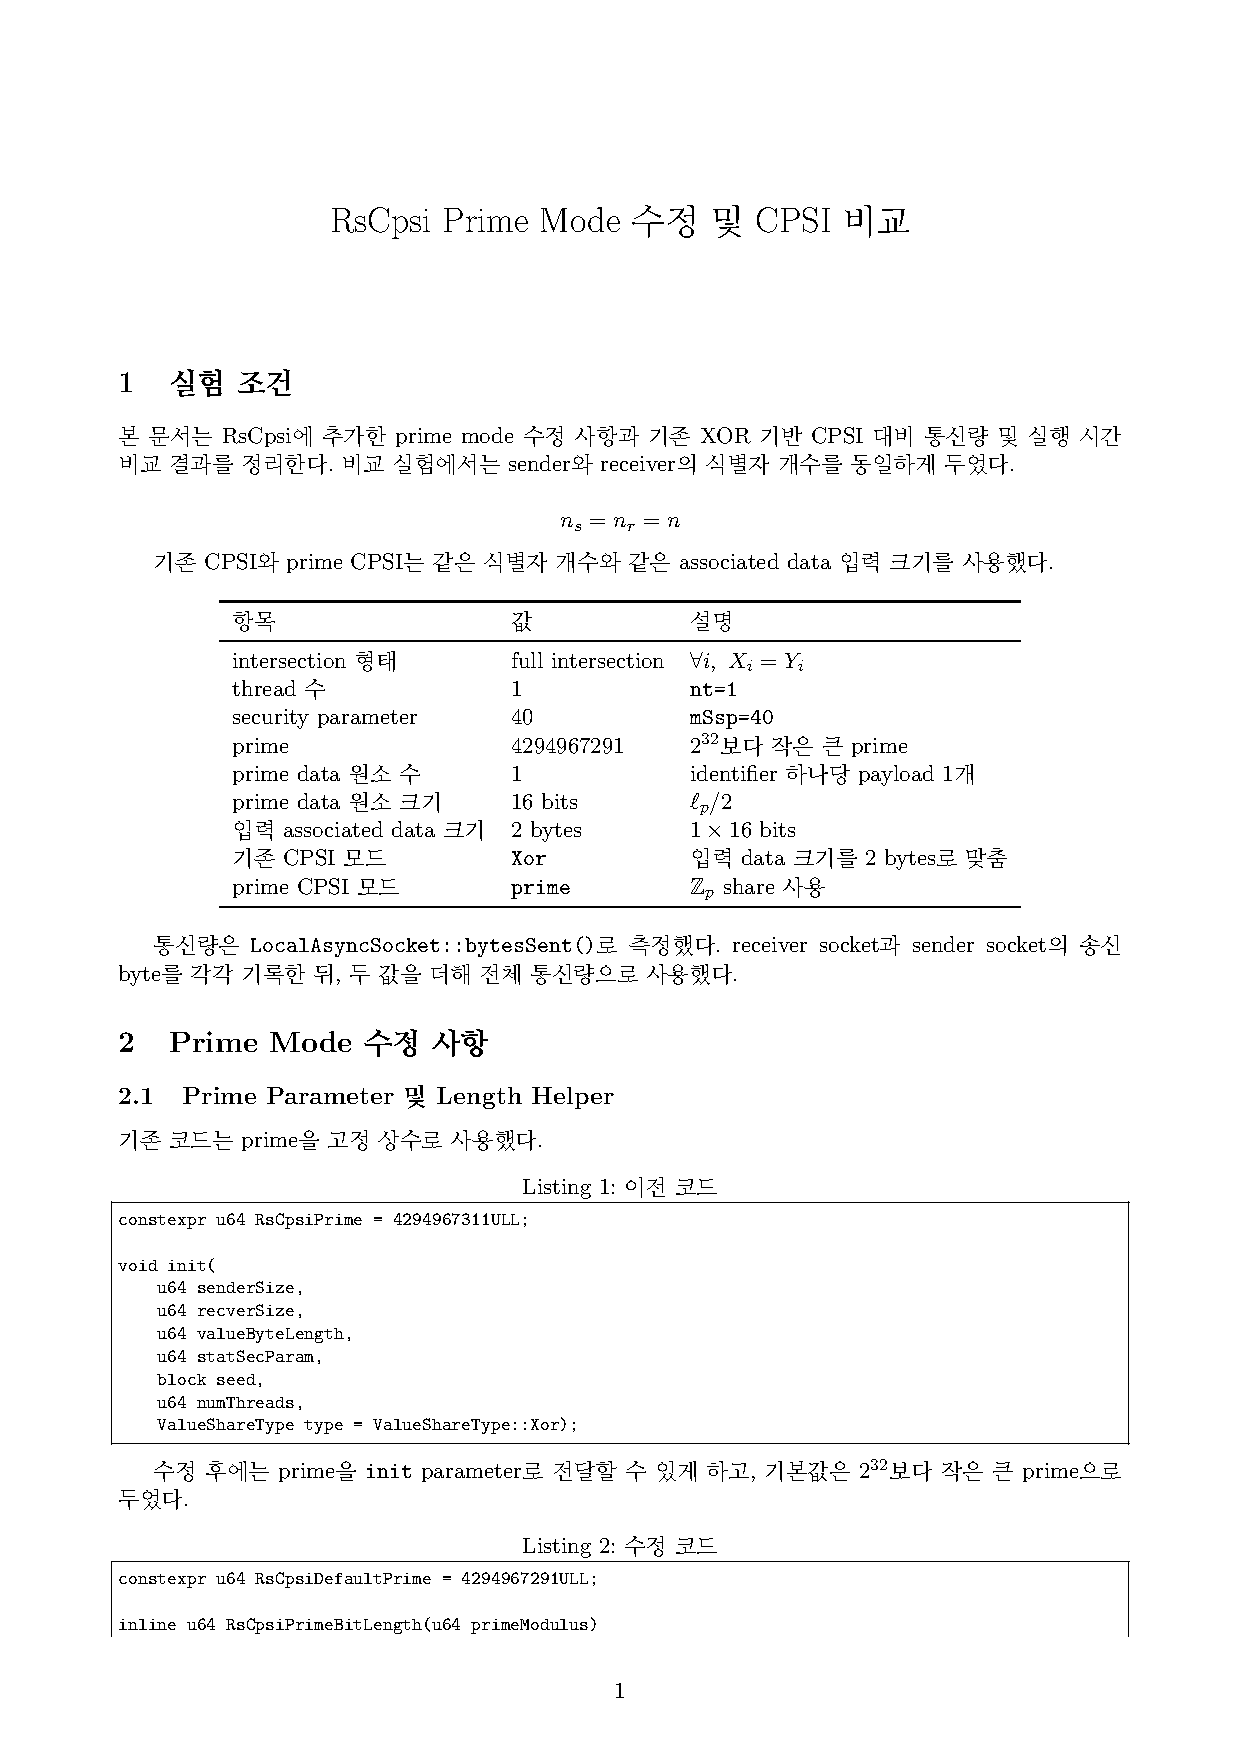
\includepdf[pages=-]{cpsi_compare_0719_original.pdf}

\clearpage
\section*{CPSI Part별 통신량 비교}

본 절에서는 \(n=2^{10}=1024\)일 때 CPSI를 실제로 한 번 실행하여,
OPRF, OPPRF, PEQT, Other part에서 발생한 통신량을 각각 측정하였다.
측정은 전체 CPSI 실행 이후 차이를 빼는 방식이 아니라, 실제 프로토콜 실행
중 각 part의 송신 구간을 직접 계측하는 방식으로 수행하였다. 따라서
아래 표의 실측값 합은 전체 CPSI 실측 통신량과 일치한다.

\subsection*{이론식}

이론적 통신량은 다음 근사식을 사용하였다. 여기서 \(n\)은 데이터 개수,
\(\ell\)은 payload 크기(bit)를 의미한다. 본 실험에서는 XOR mode의
payload를 \(16\) bit, prime mode의 payload를 \(32\) bit로 두었다.

\[
C_{\mathrm{OPRF}} = 128 \cdot 1.3n
\]

\[
C_{\mathrm{OPPRF}} = 3 \cdot 1.3n \cdot (40 + \log_2 n + \ell)
\]

\[
C_{\mathrm{PEQT}} = 4 \cdot 1.3n \cdot (40 + \log_2 n)
\]

Other part의 이론값은 cuckoo seed 전송에 해당하는 \(128\) bit로 두었다.
반면 실측값은 coproto message framing 등 실제 실행 시 발생하는 통신량을
bit 단위로 환산한 값이다.

\begin{table}[h]
\centering
\caption{Part별 이론 통신량과 XOR/prime mode 실측 통신량 비교
(\(n=2^{10}\), \(m=1305\), \(40+\log_2 m=51\) bit)}
\resizebox{\textwidth}{!}{%
\begin{tabular}{l
                S[table-format=7.1]
                S[table-format=7.1]
                S[table-format=7.0]
                S[table-format=7.0]}
\toprule
Part
& {XOR 이론 (bit)}
& {prime 이론 (bit)}
& {XOR 실측 (bit)}
& {prime 실측 (bit)} \\
\midrule
OPRF  & 170393.6 & 170393.6 & 4954712 & 4954712 \\
OPPRF & 267571.2 & 331468.8 & 299032  & 365384  \\
PEQT  & 271564.8 & 271564.8 & 1517448 & 1517448 \\
Other & 128.0    & 128.0    & 384     & 384     \\
\midrule
Total & 709657.6 & 773555.2 & 6771576 & 6837928 \\
\bottomrule
\end{tabular}
}
\end{table}

표에서 prime mode의 증가분은 주로 OPPRF value에 포함되는 payload 길이가
\(16\) bit에서 \(32\) bit로 증가한 데서 발생한다. OPRF와 PEQT는 payload
크기에 직접 의존하지 않으므로 두 mode에서 동일한 값으로 측정되었다.

\end{document}
